\documentclass{article}%
\usepackage[T1]{fontenc}%
\usepackage[utf8]{inputenc}%
\usepackage{lmodern}%
\usepackage{textcomp}%
\usepackage{lastpage}%
\usepackage{geometry}%
\geometry{margin=0.7in}%
\usepackage{ragged2e}%
\usepackage{graphicx}%
\usepackage{fancyhdr}%
%
\fancypagestyle{header}{%
\renewcommand{\headrulewidth}{0pt}%
\renewcommand{\footrulewidth}{0pt}%
\fancyhead{%
}%
\fancyfoot{%
}%
\fancyhead[L]{%
Page date: %
\linebreak%
2023{-}02{-}19%
}%
\fancyhead[C]{%
Georgia Institute of Technology%
}%
\fancyhead[R]{%
Page \thepage\ of \pageref{LastPage}%
}%
}%
%
\begin{document}%
\normalsize%
\pagestyle{header}%
\begin{minipage}{\textwidth}%
\centering%
\begin{Large}%
\textbf{HW3: Problem 1}%
\end{Large}%
\linebreak%
\begin{large}%
\textbf{Ian Dover}%
\end{large}%
\end{minipage}%
\section{Part 1}%
\label{sec:Part1}%
The relative error for the core tensor is: 0.05343890097919052.\newline%
\newline%
\newline%

%
\section{Part 2}%
\label{sec:Part2}%
Below is the relative error for each threshold:\newline%
%
percentiles,relative\_errors\newline%
0.1,0.11737302332286101\newline%
0.2,0.09141646112177233\newline%
0.3,0.07677916921832018\newline%
0.4,0.06730272837662707\newline%
0.5,0.061074384679902415\newline%
\newline%
\newline%
%


\begin{figure}[h!]%
\centering%

\includegraphics[width=120px]{/com.docker.devenvironments.code/output/Problem3/percentile_01_image_5.png}%
\caption{Percentile = 0.1; Image 5}%
\end{figure}

%


\begin{figure}[h!]%
\centering%

\includegraphics[width=120px]{/com.docker.devenvironments.code/output/Problem3/percentile_01_image_10.png}%
\caption{Percentile = 0.1; Image 10}%
\end{figure}

%


\begin{figure}[h!]%
\centering%

\includegraphics[width=120px]{/com.docker.devenvironments.code/output/Problem3/percentile_01_image_15.png}%
\caption{Percentile = 0.1; Image 15}%
\end{figure}

%


\begin{figure}[h!]%
\centering%
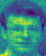
\includegraphics[width=120px]{/com.docker.devenvironments.code/output/Problem3/percentile_02_image_5.png}%
\caption{Percentile = 0.2; Image 5}%
\end{figure}

%


\begin{figure}[h!]%
\centering%

\includegraphics[width=120px]{/com.docker.devenvironments.code/output/Problem3/percentile_02_image_10.png}%
\caption{Percentile = 0.2; Image 10}%
\end{figure}

%


\begin{figure}[h!]%
\centering%

\includegraphics[width=120px]{/com.docker.devenvironments.code/output/Problem3/percentile_02_image_15.png}%
\caption{Percentile = 0.2; Image 15}%
\end{figure}

%


\begin{figure}[h!]%
\centering%
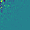
\includegraphics[width=120px]{/com.docker.devenvironments.code/output/Problem3/percentile_03_image_5.png}%
\caption{Percentile = 0.3; Image 5}%
\end{figure}

%


\begin{figure}[h!]%
\centering%

\includegraphics[width=120px]{/com.docker.devenvironments.code/output/Problem3/percentile_03_image_10.png}%
\caption{Percentile = 0.3; Image 10}%
\end{figure}

%


\begin{figure}[h!]%
\centering%

\includegraphics[width=120px]{/com.docker.devenvironments.code/output/Problem3/percentile_03_image_15.png}%
\caption{Percentile = 0.3; Image 15}%
\end{figure}

%


\begin{figure}[h!]%
\centering%
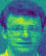
\includegraphics[width=120px]{/com.docker.devenvironments.code/output/Problem3/percentile_04_image_5.png}%
\caption{Percentile = 0.4; Image 5}%
\end{figure}

%


\begin{figure}[h!]%
\centering%

\includegraphics[width=120px]{/com.docker.devenvironments.code/output/Problem3/percentile_04_image_10.png}%
\caption{Percentile = 0.4; Image 10}%
\end{figure}

%


\begin{figure}[h!]%
\centering%

\includegraphics[width=120px]{/com.docker.devenvironments.code/output/Problem3/percentile_04_image_15.png}%
\caption{Percentile = 0.4; Image 15}%
\end{figure}

%


\begin{figure}[h!]%
\centering%

\includegraphics[width=120px]{/com.docker.devenvironments.code/output/Problem3/percentile_05_image_5.png}%
\caption{Percentile = 0.5; Image 5}%
\end{figure}

%


\begin{figure}[h!]%
\centering%
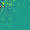
\includegraphics[width=120px]{/com.docker.devenvironments.code/output/Problem3/percentile_05_image_10.png}%
\caption{Percentile = 0.5; Image 10}%
\end{figure}

%


\begin{figure}[h!]%
\centering%

\includegraphics[width=120px]{/com.docker.devenvironments.code/output/Problem3/percentile_05_image_15.png}%
\caption{Percentile = 0.5; Image 15}%
\end{figure}

%
\end{document}